\documentclass[10pt]{beamer}
\usepackage[utf8]{inputenc}

\usepackage{graphicx}
\usepackage{listings}
\usepackage{tabu}

\newcommand{\code}[1]{\texttt{#1}}

\usetheme{Madrid}
%\usetheme{boxes}
%\usetheme{Singapore}
%\usetheme{Pittsburgh}

\usecolortheme{whale}
%\usecolortheme{dove}
%\usecolortheme{lily}
\usecolortheme{orchid}

\title{An educational kernel for the Raspberry Pi}
\subtitle{CS310 - Presentation}
\author{Thomas Archbold}
\date{\today}

\begin{document}

\begin{frame}
    \titlepage
\end{frame}

\begin{frame}{Introduction}

\begin{columns}[c]
    \column{.5\textwidth}
    Operating systems are some of the most pervasive pieces of software around,
    but also some of the most complex \\~\\

    The introduction of the Raspberry Pi has made computers much more accessible
    - allows and encourages experimenting at all levels \\~\\

    There are several official operating systems for the Pi - NOOBS, Raspbian,
    Windows IoT core, PiNET - but none provide a resource to learn about the
    operating system itself

    \column{.5\textwidth}
    \begin{figure}
        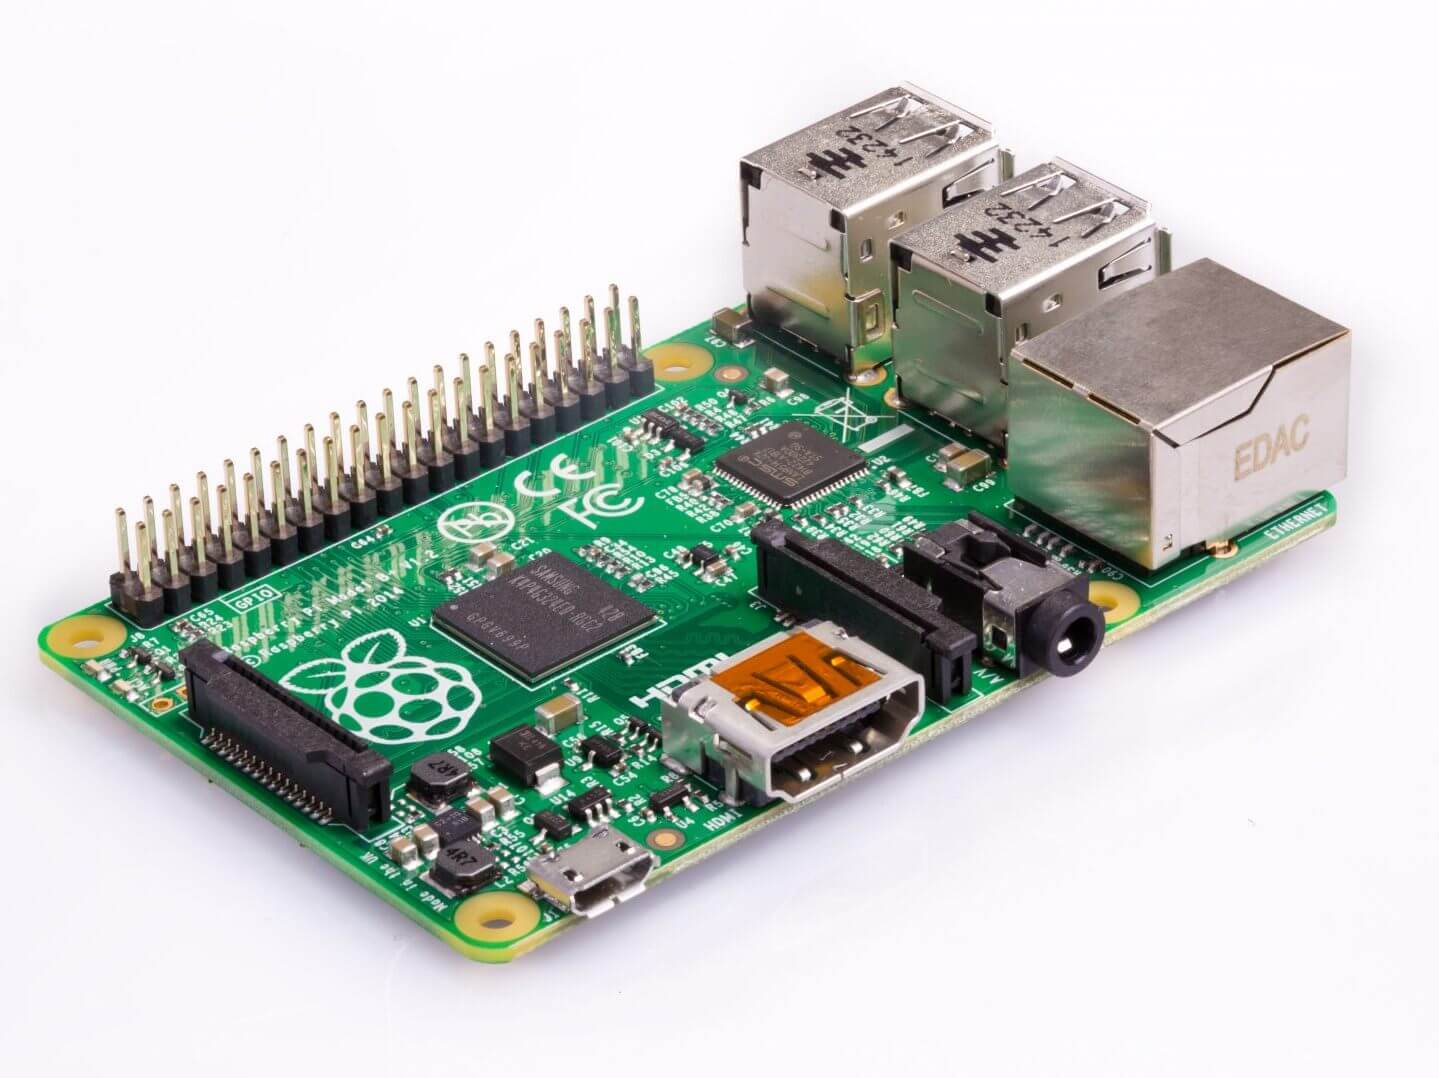
\includegraphics[width=\linewidth]{raspi1B.jpg}
    \end{figure}
\end{columns}

\end{frame}

\begin{frame}{Objectives}
    \textbf{Main goal:}
    to write a configurable operating system for the Raspberry Pi capable of
    booting on real hardware for educational and hobbyist use. \\~\\

    Specifically, this involves:
    \begin{itemize}
        \item providing different approaches for tasks such as scheduling,
            interprocess communication, and permanent storage
        \item allowing the user to configure the system at compile time to use
            different combinations of these approaches, and
        \item exposing a simple and easily extensible interface for additional
            features
    \end{itemize}
\end{frame}

\begin{frame}{Background material}
    \begin{itemize}
        \item Pintos - Stanford's instructional x86 operating system, used to
            teach their CS140 course
        \item Baking Pi - Cambridge's tutorial on writing an operating system
            for the Raspberry Pi in assembly
        \item MINIX - Tanenbaum and Woodhull's illustrative operating system for
            ``Operating Systems: Design and Implementation''
        \item The little book about OS development - Helin and Renberg's
            ``practical guide to writing your own x86 operating system''
        \item \url{osdev.org/} - community of hobbyist operating system
            developers, containing information, tutorials, advice, etc.
    \end{itemize}
\end{frame}

\begin{frame}{Why is this project worthwhile?}
\centering
    It is more difficult to get into low-level/systems programming \\
    $\Rightarrow$ focus is on clear code to aid understanding \\~\\

    The project attempts to demystify aspects of operating system development -
    able to see the theory in practise \\~\\

    It will provide an accessible platform to further tinker and experiment with
    operating system development, with little to lose
\end{frame}

\begin{frame}{Useful concepts - compilation}
    \only<1>{
    \textbf{Operating System} - program that manages a computer's hardware \\~\\
    \textbf{Freestanding environment} - little access to C standard library, and
    program entry point not necessarily at \texttt{main()} \\ $\quad
    \Rightarrow$ must implement most of standard library ourselves \\~\\
    \textbf{Cross-compiler} - allows us to compile code that will run on the
    target architecture from our own machine \\~\\
    \textbf{Linker} - responsible for linking all compiled \texttt{.o} files
    into one executable \\
    Defines the following sections:
    \begin{itemize}
        \item \code{.text} - executable code
        \item \code{.rodata} read-only data (i.e. global constants)
        \item \code{.data} - global variables that are itialised at compile-time
        \item \code{.bss} - uninitialised global variables
    \end{itemize}
    }

    \only<2>{
    \begin{figure}
        \centering
        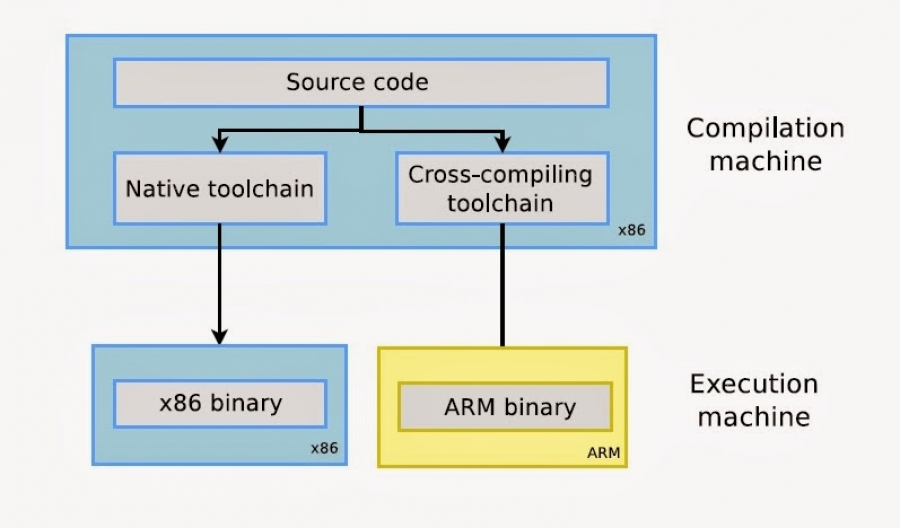
\includegraphics[width=.8\textwidth]{cross-compiler.jpg}
        \caption{Cross-compilation}
    \end{figure}
    }
\end{frame}

\begin{frame}{Useful concepts - general}
    \textbf{Kernel} - the core of the operating system; the one program which is
    running at all times throughout execution \\

    \textbf{Exception} - an event triggered when something exceptional happens
    during normal execution (hardware giving CPU data, privileged action, bad
    instruction) \\

    \textbf{Process} - a program that has been loaded into memory and is
    executing \\

    \textbf{Concurrency} - the ability for multiple processes to make progress
    seemingly simultaneously, as a result of some scheduling algorithm \\

    \textbf{Context Switch} - switching execution to another process. Involves:
    \begin{enumerate}
        \item saving the state of the currently executing process (\textbf{state
            save})
        \item loading the saved state of a different process (\textbf{state
            restore})
    \end{enumerate}
\end{frame}

\begin{frame}{Useful concepts - general contd.}
    \textbf{Synchronisation} - the prevention of \textbf{race conditions}: when
    the outcome of two concurrently executing processes depends on the order in
    which data access took place \\

    \textbf{Interprocess Communication} - mechanism by which cooperating
    processes may exchange data and information

    \begin{figure}[h]
        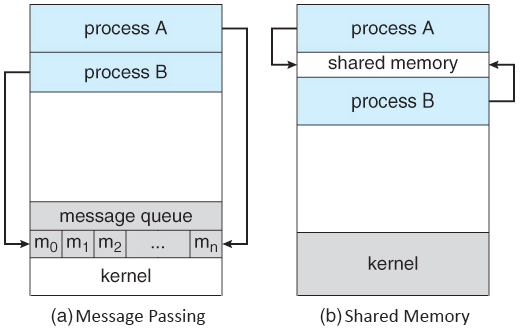
\includegraphics[width=.5\textwidth]{ipc.png}
        \caption{The two fundamental models of interprocess communication}
    \end{figure}
\end{frame}

\begin{frame}{Useful concepts - Pi specific}
    \textbf{Peripheral} - a device with a specific address that it may read and
    write data to and from
    \begin{itemize}
        \item All peripherals may be described by an offset from the Peripheral
            Base Address (\code{0x20000000} on the Raspberry Pi 1 Model B+)
        \item Peripherals include: timers, interrupt controller, GPIO, USB, UART
    \end{itemize} ~

    \textbf{Memory Mapped I/O} - uses same address space to address both memory
    and I/O devices $\Rightarrow$ the memory and registers of the I/O devices
    are mapped to address values
    \begin{itemize}
        \item e.g. to turn the ACT LED on, we simply write a bit at the correct
            offset: \code{mmio\_write(ACT\_GPSET, 1 << ACT\_GPBIT)}
        \item where \code{mmio\_write()} is simply \code{*(volatile uint32\_t *)
            reg = data;}
    \end{itemize}
\end{frame}

\begin{frame}{Tools used}
    Languages: C and ARM assembly \\~\\
    Cross-compiler toolchain: \texttt{arm-none-eabi} \\~\\
    Build automation: Make \\~\\
    Version control: git \\~\\
    Emulation: QEMU \\~\\
    Model: Raspberry Pi 1 Model B+
\end{frame}

\begin{frame}{Raspberry Pi 1 Model B+}
    \begin{columns}
    \column{.5\textwidth}
        \textbf{Hardware}
        \begin{itemize}
            \item System-on-Chip (SoC): BCM2835
            \item CPU: 700MHz ARM1176JZF-6
            \item GPU: 250MHz Broadcom VideoCore IV
            \item Memory: 512MiB
            \item USB: 4x USB 2.0 ports
            \item Video output: HDMI
            \item Peripherals: 40 GPIO pins, UART
            \item Storage: MicroSD card
        \end{itemize}

    \column{.5\textwidth}
        \begin{figure}[h]
            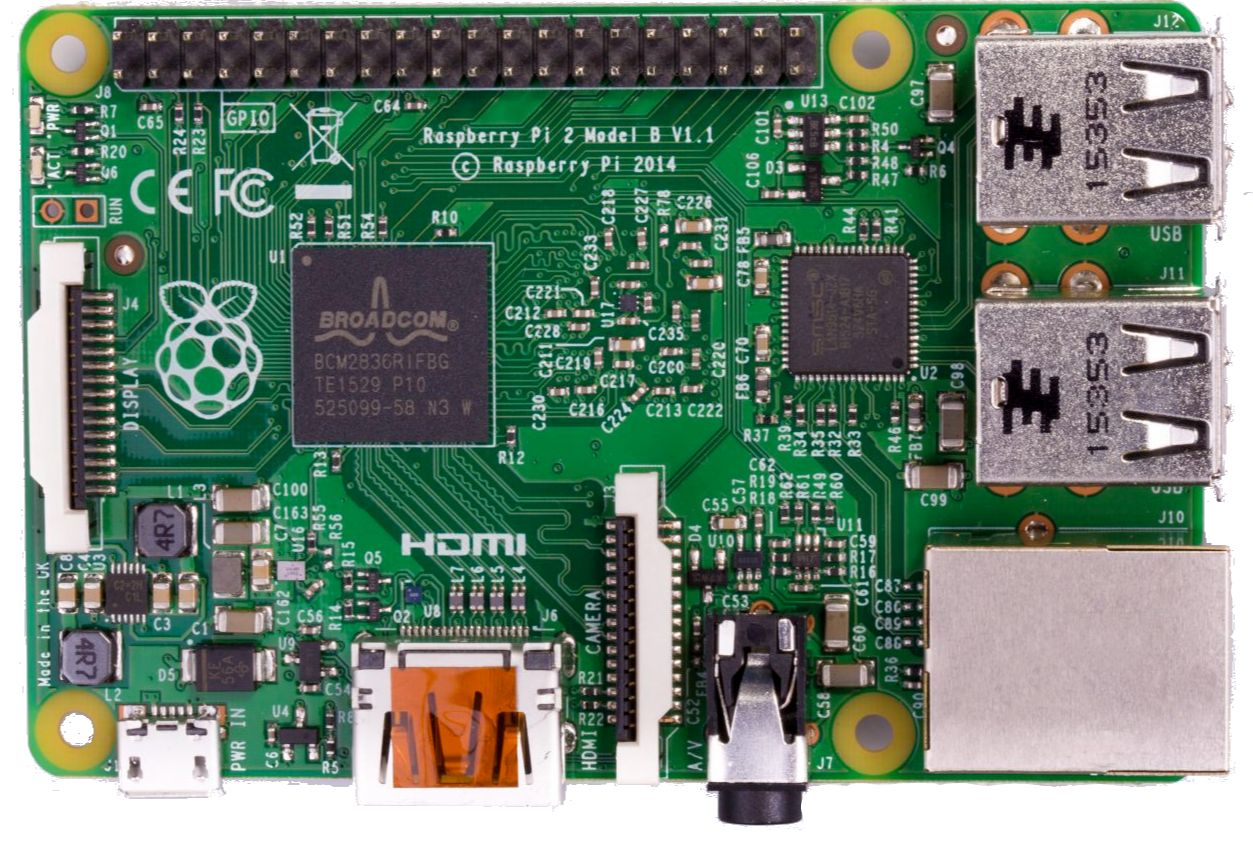
\includegraphics[width=.8\textwidth]{raspi.png}
        \end{figure}
    \end{columns} ~\\

    % or \only
    \onslide<2->{\textbf{Why the Pi in particular?}} \\
    \onslide<3->{Simple boot process - handled entirely by SoC} \\
        \onslide<4->{Underlying architecture of BCM2835 chip is identical to
        BCM2836/7} \\
        \onslide<5->{Standard set of hardware $\Rightarrow$ more widely
        accessible}
\end{frame}

\begin{frame}{Project overview}
    Main milestones reached:
    \begin{itemize}
        \item Capable of booting in emulated environment
        \item Capable of booting on real hardware
        \item Display on real screen through HDMI
        \item Interrupts
        \item Processes and Threads
        \item Concurrency
        \item Synchronisation
    \end{itemize} ~\\

    \textbf{Current goal:} interprocess communication
\end{frame}

\begin{frame}{Project management - organisation}
    Project has been developed more-or-less with a waterfall-style approach
    \begin{itemize}
        \item rigidity of (early) system lends itself well to this
    \end{itemize} ~
    Project only now beginning to open up more \\

    Term 1:
    \begin{itemize}
        \item reading technical documentation (Technical Reference Manuals,
            etc.)
        \item barebones kernel followed by extension
        \item ended term having written dynamic memory allocator (\code{kmalloc,
            kfree}
    \end{itemize} ~

    Term 2:
    \begin{itemize}
        \item HDMI output up to concurrency and synchronisation achieved
    \end{itemize} ~

    Despite progress, somewhat behind schedule
    \begin{itemize}
        \item Certain amount of underestimation - lack of experience
    \end{itemize}
\end{frame}

\begin{frame}{Project management - testing}
    Fortnightly supervisor meetings held in Term 1 - higher course load \\~\\
    Increased to weekly meetings - focus shifted more towards project \\

    \textbf{Testing} \\
    Almost entirely manual - exists little infrastructure to debug \\
    In most early cases this was done through blinking the ACT LED \\
    $\Rightarrow$ vital to implement \code{printf()} soon after printing to HDMI
    \\

    Incremental/waterfall approach has helped in this regard
    \begin{itemize}
        \item once a feature is complete, can be left fairly untouched
    \end{itemize}
\end{frame}

\begin{frame}{Design overview}
    \begin{figure}
        \centering
        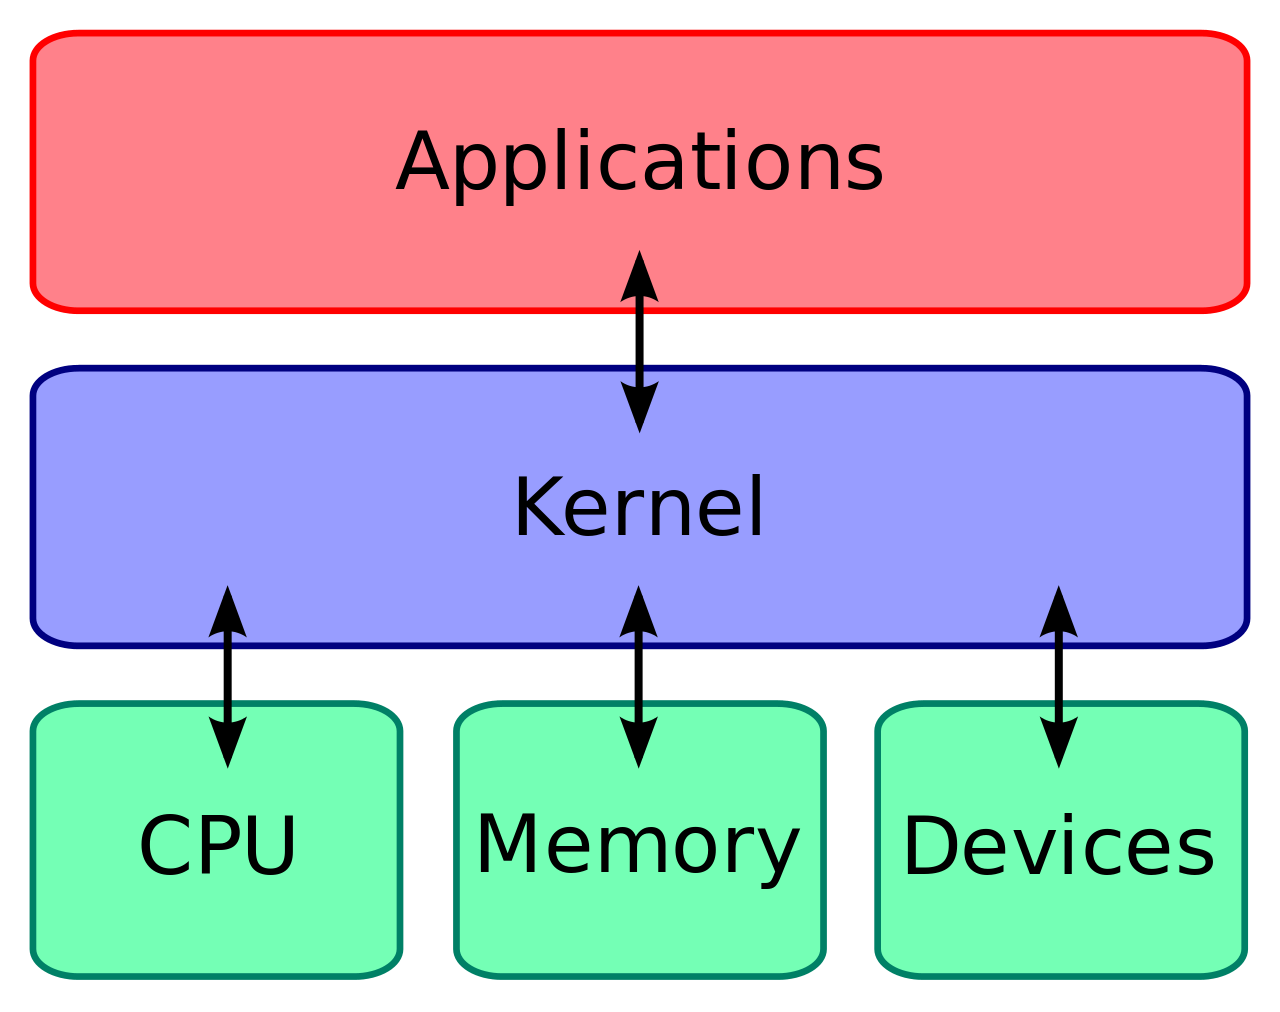
\includegraphics[width=.8\textwidth]{kernel.png}
    \end{figure}
\end{frame}

\begin{frame}[fragile]
    \frametitle{Design overview - boot}
    \textbf{Booting}
    \begin{itemize}
        \item Bootloading handled by SoC, so just need to set up system and
            initialise C runtime
        \item \texttt{boot.S} initialises stack pointer at \texttt{0x8000},
            zeroes \texttt{bss} segment, then loads C kernel entry point
            \texttt{kernel\_main()} to begin execution
    \end{itemize} ~

    \textbf{Memory management - atags}
    \begin{itemize}
        \item Bootloader creates list of information about the hardware called
            \textbf{atags}
        \item Each tag consists of a header and tag-specific data
        \item To find the amount of memory available to the system, simply
            iterate over list of tags until the \texttt{tag == ATAG\_MEM}, at
            which point return \texttt{atag\_mem.size}
    \end{itemize}

    \begin{columns}[t]
    \column{.6\textwidth}
        \lstset{language=C,basicstyle=\ttfamily}
        \begin{lstlisting}
enum atag_tag {
    ATAG_NONE = 0x00000000,
    ATAG_CORE = 0x54410001,
    ATAG_MEM  = 0x54410002,
    ...
};
        \end{lstlisting}
    \column{.35\textwidth}
        \lstset{language=C,basicstyle=\ttfamily}
        \begin{lstlisting}
struct atag_mem {
    uint32_t size;
    uint32_t start;
};
        \end{lstlisting}
    \end{columns}
\end{frame}

\begin{frame}{Design overview - memory}
    \onslide<1->{
    \textbf{Memory - paging}
    \begin{itemize}
        \item Memory split into 4kiB pages
        \item Each page contains metadata (allocated, kernel page, kernel heap
            page, shared), metadata for \code{all\_pages} stored just after
            \code{\_\_end}
        \item Maintain two lists: \code{all\_pages} and \code{free\_pages}
        \item Allocating and freeing pages - simply dequeue/append page to
            \code{free\_pages} and alter flags
    \end{itemize}
    }

    \onslide<2->{
    \textbf{Memory - heap}
    \begin{itemize}
        \item 1MiB reserved after page metadata for the heap
        \item Associate each allocation with header and store in linked list
        \begin{itemize}
            \item allocation size
            \item ``in-use'' flag
        \end{itemize}
        \item \code{kmalloc(bytes)} - traverse list to find best-fitting unused
            segment
        \item \code{kfree(ptr)} - unset \code{allocated} bit and coalesce
            adjacent segments
    \end{itemize}
    }
\end{frame}

\begin{frame}[fragile]
    \frametitle{Design overview - HDMI output}

    \textbf{Printing to screen} \\
    Must ask GPU for \textbf{framebuffer} - piece of memory shared between CPU
    and GPU \\
    Process differs slightly between Pi 1 and Pi 2 - both use the mailbox
    peripheral
    \begin{itemize}
        \item Pi 1 - uses framebuffer mailbox channel
        \item Pi 2 - uses property mailbox channel (more abstract)
    \end{itemize}

    \begin{columns}
    \column{.4\textwidth}
        \lstset{language=C,basicstyle=\ttfamily}
        \begin{lstlisting}
struct fb_init {
    uint32_t width;
    uint32_t height;
    uint32_t v_width;
    uint32_t v_height;
    uint32_t bytes;
    uint32_t depth;
    uint32_t ignore_x;
    uint32_t ignore_y;
    void    *pointer;
    uint32_t size;
};}
        \end{lstlisting}

    \column{.5\textwidth}
        \textbf{Asking for a framebuffer:}
        \begin{itemize}
            \item Set desired framebuffer attributes by initialising
                \code{fb\_init}
            \item Send 16-byte aligned structure as message through framebuffer
                mailbox to GPU
            \item On success, initialise \code{fb\_info} struct using values
                from \code{fb\_init}
        \end{itemize}
    \end{columns}
\end{frame}

\begin{frame}[fragile]
    \frametitle{Design overview - framebuffer}
    \begin{columns}
    \column{.5\textwidth}
        \begin{itemize}
            \item Pitch - number of bytes on each row of the screen
            \item Depth - number of bits per pixel
        \end{itemize}

    \column{.5\textwidth}
        \lstset{language=C,basicstyle=\ttfamily}
        \begin{lstlisting}
struct framebuffer_info {
    uint32_t width;
    uint32_t height;
    uint32_t pitch;
    void    *buffer;
    uint32_t bufsize;
    uint32_t max_col;
    uint32_t max_row;
    uint32_t col;
    uint32_t row;
};
        \end{lstlisting}
    \end{columns}

\end{frame}

\begin{frame}{Design overview - interrupts}
    \textbf{Interrupts and Exceptions} \\
    \onslide<1->{
        When an exception occurs, a specific address is loaded into the Program
        Counter \\
        Branch instructions must be written at these locations to branch to
        correct exception-handling routines
    }

    \onslide<2->{
    \begin{center}
        \begin{tabu} to \textwidth { |c|l|X[l]| }
         \hline
\textbf{Address} & \textbf{Exception} & \textbf{Source}  \\ \hline
0x00 & Reset & Hardware reset \\ \hline
0x04 & Undefined instruction & Executing garbage instruction \\ \hline
0x08 & Software Interrupt (SWI) & Software wants to execute privileged operation \\ \hline
0x0c & Prefetch Abort & Bad memory access of instruction \\ \hline
0x10 & Data Abort & Bad memory access of data \\ \hline
0x14 & Reserved & Reserved \\ \hline
0x18 & Interrupt Request (IRQ) & Hardware telling CPU something \\ \hline
0x1c & Fast Interrupt Request (FIQ) & Piece of hardware can do this faster than all others \\ \hline
        \end{tabu}
    \end{center}
    }

\end{frame}

\begin{frame}{Design overview - IRQs}
    Exception handlers are functions, but not normal ones \\
    \onslide<2->{
        $ \quad \Rightarrow$
        \code{void \_\_attribute\_\_((interrupt("ABORT"))) reset\_handler(void);}
    } \\

    \textbf{IRQ peripheral} used to determine device that triggered IRQ
    \begin{itemize}
        \item located at offset \code{0xb000} from peripheral base address
    \end{itemize} ~

    IRQ peripheral registers:
    \begin{itemize}
        \item Pending - indicate whether a given interrupt has triggered
        \item Enable - enable certain interrupts by setting appropriate bit
        \item Disable - disable certain interrupts by setting appropriate bit
    \end{itemize} ~

    Pi has 72 possible IRQs
    \begin{itemize}
        \item 0-63 are shared by CPU and GPU
        \item 64-71 are specific to CPU
    \end{itemize} ~

    Timer is IRQ 1, USB controller is IRQ 9
\end{frame}

\begin{frame}{Design overview - System Timer}
    QEMU does not simulate a system timer, at least for the Raspberry Pi \\
    $ \quad \Rightarrow$ at this point it is vital to switch to real hardware \\

    The system timer is a hardware clock which can keep time and generate
    interrupts after a certain time
    \begin{itemize}
        \item starts when Pi boots and increments 64-bit counter every
            microsecond
        \item it is a peripheral that is located at offset \code{0x3000} from
            peripheral base
    \end{itemize} ~

    Four registers which the timer compares the low 32 bits with each counter
    tick
    \begin{itemize}
        \item if any compare register matches the counter, an IRQ is triggered
    \end{itemize} ~

    Timer is set by setting \code{compare1} register to the current value plus
    some number of microseconds
\end{frame}

\begin{frame}{Design overview - Processes}
    \textbf{Process Control Block (PCB)} - structure which holds all of the
    information about a process
    \begin{itemize}
        \item State save is done simply by pushing all of the registers onto the
            stack
    \end{itemize} ~

    We maintain two lists:
    \begin{itemize}
        \item job queue - holds all processes in the system
        \item ready queue - holds all processes residing in main memory and
            waiting to execute
    \end{itemize} ~

    Creating a new process as simple as allocating space for PCB and process'
    stack and adding it to the ready queue
    \begin{itemize}
        \item simple interface: \\
        \code{void create\_kthread(kthreadfn func, char *name, int name\_len);}
    \end{itemize}
\end{frame}

\begin{frame}[fragile]
    \frametitle{Design overview - PCB}

    \begin{columns}
    \column{.5\textwidth}
        \lstset{language=C,basicstyle=\ttfamily}
        \begin{lstlisting}
struct proc_state {
    uint32_t r0;
    uint32_t r1;
    uint32_t r2;
    uint32_t r3;
    uint32_t r4;
    uint32_t r5;
    uint32_t r6;
    uint32_t r7;
    uint32_t r8;
    uint32_t r9;
    uint32_t r10;
    uint32_t r11;
    uint32_t cpsr;
    uint32_t sp;
    uint32_t lr;
};
        \end{lstlisting}

    \column{.5\textwidth}
        \lstset{language=C,basicstyle=\ttfamily}
        \begin{lstlisting}
struct proc {
    struct proc_state *state;
    uint32_t pid;
    char name[32];
    void *stack_page;
    DEFINE_LINK(proc);
};
        \end{lstlisting}
    \end{columns}

\end{frame}

\begin{frame}{Design overview - scheduling}
    Processes have no consideration for other processes
    \begin{itemize}
        \item if they could they would hog the entire CPU until they are done
    \end{itemize}
    $ \Rightarrow$ we have to systematically kick them off the CPU \\

    \textbf{Round Robin}
    \begin{itemize}
        \item each process given a set quantum of time to use CPU
        \item CPU use then given to another waiting process, regardless of
            process' progress
    \end{itemize}
    \begin{figure}
        \centering
        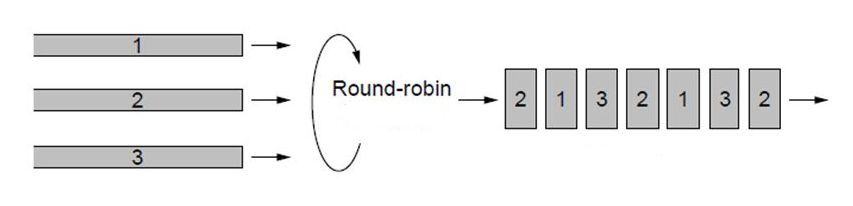
\includegraphics[width=.8\textwidth]{round_robin.jpg}
    \end{figure}
\end{frame}

\begin{frame}[fragile]
    \frametitle{Design overview - context switch}
    To switch between processes, we must perform a \textbf{context switch}
    \begin{itemize}
        \item save process' registers and stack pointer
        \item load saved stack pointer of next process and pop registers
    \end{itemize}

    \begin{columns}
    \column{.4\textwidth}
        \code{switch\_context(old, new)}:
        \lstset{language=C,basicstyle=\ttfamily}
        \begin{lstlisting}
    str sp, [r0]
    ldr sp, [r1]
        \end{lstlisting}

    \column{.5\textwidth}
        \begin{figure}
            \centering
            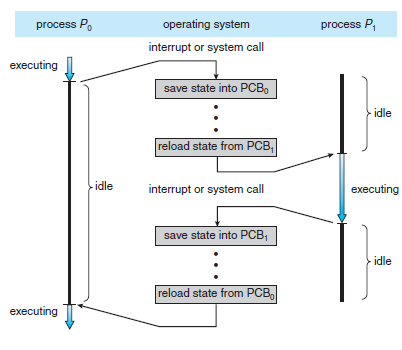
\includegraphics[width=\textwidth]{context_switch.png}
        \end{figure}
    \end{columns}

    We also set the timer to go off in another quantum
\end{frame}

\begin{frame}[fragile]
    \frametitle{Design overview - synchronisation}
    With concurrency, there is the opportunity for race-conditions \\

    We use the concept of an \textbf{atomic swap} to implement spinlocks and
    mutexes - cannot be preempted while trying to take lock

    \lstset{language=C,basicstyle=\ttfamily}
    \begin{lstlisting}
if (lock == 1)
    lock = 0;
    \end{lstlisting}

    The problem is that it can be preempted while checking \code{lock} value
    \begin{itemize}
        \item instead, check if we got the lock after taking it
    \end{itemize} ~

    \textbf{Spinlock} - try to acquire lock in loop until successful \\
    \textbf{Mutex lock} - maintain list of processes that want it
\end{frame}

\begin{frame}[fragile]
    \frametitle{Configuration}
    Configuration done at compile-time
    \begin{itemize}
        \item based on command-line arguments, send different directives \\
        e.g. \code{make model=1 sched=roundrobin} \\
        $\Rightarrow$ \code{DIRECTIVES = -DRPIBPLUS -DSCHED\_ROUNDROBIN}
    \end{itemize} ~

    Once interprocess communication is implemented, this will similarly
    configured
\end{frame}

\begin{frame}{Next steps}
    Currently working on:
    \begin{itemize}
        \item keyboard input and shell
        \item interprocess communication
    \end{itemize} ~

    After this, the final core feature will be permanent storage i.e.
    filesystems and interacting with microSD card
\end{frame}

\begin{frame}{Evaluation}
    Overall the project has been success - despite the difficulty in sticking to
    schedule, much progress has been made \\

    Gained a lot of experience in systems programming
    \begin{itemize}
        \item process (preprocessing, compilation, linking)
        \item C and ARM competency improved (ability to switch between \code{.S}
            and \code{.c}, more advanced C)
        \item confidence in Make (conditional compilation, well-structured)
        \item ability to digest technical documentation (deep knowledge of Pi
            required)
    \end{itemize}
\end{frame}

\begin{frame}{Evaluation}
    \begin{columns}
    \column{.5\textwidth}
        Focus has somewhat shifted from modularity to educational
        \begin{itemize}
            \item kernel currently monolithic - no user space to speak of
            \item compile-time configuration emulates modularity to an extent
            \item truly modular kernel would have been much more complex
        \end{itemize} ~

        Operating system beginning to look like one you might use day-to-day \\

    \column{.5\textwidth}
        \begin{figure}
            \centering
            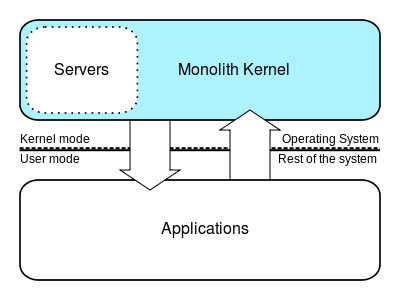
\includegraphics[width=.9\textwidth]{monolithic.png}
        \end{figure}
    \end{columns}

\end{frame}

\begin{frame}{Questions}
    \centering
    Thank you for listening
\end{frame}

\end{document}
